%% template for IEICE Transactions
%% v1.8 [2011/12/16]
\documentclass[paper]{ieice}
%\documentclass[invited]{ieice}
%\documentclass[survey]{ieice}
%\documentclass[invitedsurvey]{ieice}
%\documentclass[review]{ieice}
%\documentclass[tutorial]{ieice}
%\documentclass[letter]{ieice}
%\documentclass[brief]{ieice}
\usepackage[dvips]{graphicx}
\usepackage[fleqn]{amsmath}
\usepackage[varg]{txfonts}
\usepackage{algorithm}
\usepackage{multirow}
\usepackage{algorithmic}
\usepackage{subfig}

\setcounter{page}{1}
%\breakauthorline{}% breaks lines after the n-th author

\field{D}
%\SpecialIssue{}
%\SpecialSection{}
%\theme{}
\title{AVCS: Adaptive Virtual Channel Sharing Router Architecture for Networks-on-Chip}
%\title[title for header]{title}
%\titlenote{This research is supported by High Technology Research and Development Program of China (Grant No. 2012AA012201, 2012AA011902).}
\authorlist{% fill arguments of \authorentry, otherwise error will be caused.
 \authorentry[libaoliang@nudt.edu.cn]{Baoliang LI}{s}{label1}
 \authorentry{Quanyou Feng}{n}{label1}
 \authorentry{Wenhua DOU}{n}{label1}
% \authorentry{name}{membership}{affiliate label}
% \authorentry{name}{membership}{affiliate label}[present affiliate label]
% \authorentry[e-mail address]{name}{membership}{affiliate label}
% \authorentry[e-mail address]{name}{membership}{affiliate label}[present affiliate label]
}
\affiliate[label1]{The authors are with the College of Computer, National University of Defense Technology, China.}
%\paffiliate[present affiliate label]{Presently, the author is with the }

\received{2014}{12}{25}
%\revised{2014}{01}{8}
%\finalreceived{2011}{1}{1}

%% <local definitions here>

%% </local definitions here>

\begin{document}
\maketitle
\begin{summary}
The performance and hardware cost of wormhole-switched Networks-on-Chip (NoC) router heavily depend on the organization and management scheme of input buffer. In order to achieve high performance without introducing significant power and area burden, the management of buffer resources should adapt the dynamical change of traffic load. In this paper, we propose an inter-port Adaptive Virtual Channel (VC) Sharing router architecture, i.e. AVCS, which adjusts the VC number and buffer capacity each input port can use to improve the buffer utilization and network performance. Another contribution of this paper is that we introduce the idea of port sharing while implementing the VC Allocator (VCA) and SWitch Allocator (SWA), which utilizes a smaller VCA and SWA to meet the demand of large-scale VC and switch allocation. Based on a detailed RTL implementation, we evaluate the performance and hardware overhead of our proposal. Experimental results show that the proposed architecture saves 32.1\% power and 11.7\% chip area when compared with the typical router architecture with similar performance.
\end{summary}
\begin{keywords}
Networks-on-Chip (NoC), VC sharing, buffer utilization
\end{keywords}

\section{Introduction}
The wormhole-switched Networks-on-Chip (NoC) provides a scalable, high-performance and low-cost interconnection fabric for the large-scale Chip-MultiProcessor (CMP) and System-on-Chip (SoC). The performance, power and area of NoC router heavily depend on the buffer capacity and organization scheme. In a typical router \cite{DaTo01}, all the input ports have the same number of VCs and each VC is designated a fixed buffer capacity. Although the static structure eases hardware implementation, the buffer resources can not be fully utilized under some nonuniform traffic pattern. For the input ports with low traffic load, few buffer slots are enough to temporarily accommodate all the incoming flits that cannot be forwarded immediately, leaving the rest buffer resources of the same input port underutilized. In contrast, many buffer slots are necessary for the input ports with high traffic load to guarantee throughput. Since the buffer consumes more than 60\% power and chip area in a typical router \cite{1650108}\cite{ChPe03}, reserving large enough buffer space for each input port to ensure the performance under high traffic load is infeasible.

The only way to implement a high-performance and low-cost NoC router is by improving the buffer utilization through appropriate buffer organization and management scheme. There have been significant works on this issue, e.g. \cite{NPKV06,4555894,6310960}. To improve buffer utilization, these approaches dynamically allocate buffer slots to each VC within an input port according to the traffic condition, which can achieve 50\% buffer saving without degenerating the network performance \cite{NPKV06}. In \cite{Neishaburi:2009:RAN:1531542.1531658}\cite{5770788},
inter-port buffer sharing scheme was proposed to further improve the performance and buffer utilization of typical router. Although all these approaches employ dynamical buffer management, the number of VCs each input port can use is fixed. We find that, these approaches can not fully exploit network performance with limited buffer resources under some scenarios. We take a $3\times 3$ mesh network employing Dimension Order Routing (DOR) as an example to illustrate one of these special cases, as shown in Fig. \ref{vcensuficent}. Packets from router 9 and 3 to router 5 are blocked due to lack of available VCs at North (N) and South (S) port of router 5. Whereas, 4 VCs in total at input port West (W), East (E) and Local (L) are idle. This example reveals that only sharing buffer resources among VCs and ports is not enough to maximize the performance of wormhole-switched NoC router, because the limited VC resources restrict the usage of buffer.
\begin{figure}
  \centering
  \subfloat[All-to-1 Communication]{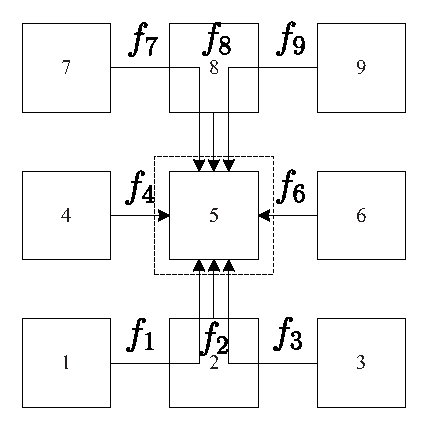
\includegraphics[scale=0.51]{figures/center.eps}\label{center}}\hspace{10pt}
  \subfloat[VC Status of Router 5]{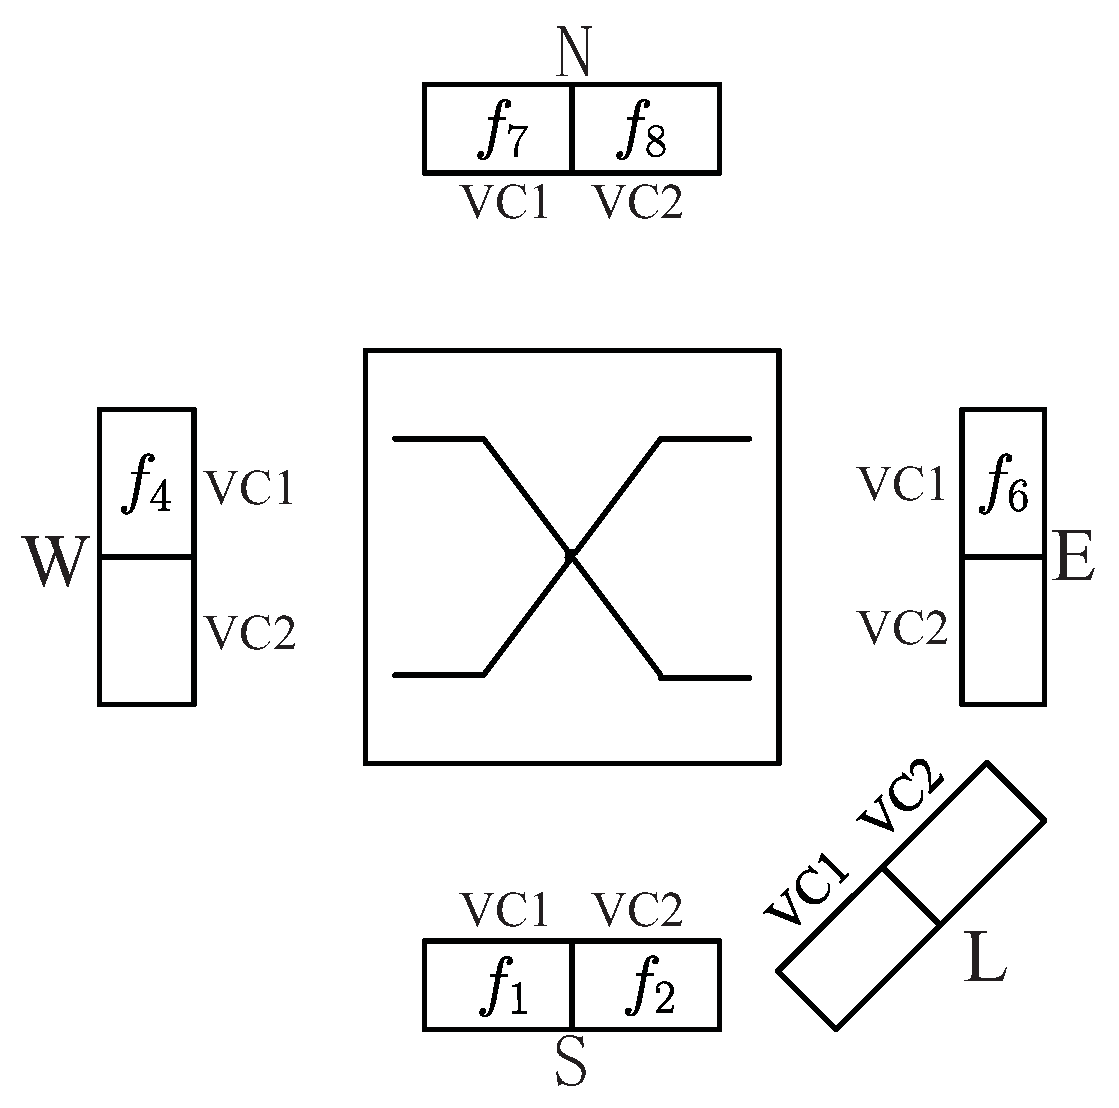
\includegraphics[scale=0.20]{figures/vcensufficient.eps}\label{vcunbalance}}
  \caption{Blocking caused by VC insufficiency}\label{vcensuficent}
\end{figure}

Since the number of VCs an input port required at any time instance is equal to the number of partial packets it accommodates, the VC resources required at each input port changes dynamically with time and traffic pattern. To avoid the blocking caused by VC insufficiency and guarantee the worst-case VCs requirement, an intuitive solution is that reserving large amount of VCs at each port. However, this solution is infeasible due to the follow two reasons: First, it introduces significant hardware overhead to manage and keep the status of each VC. Second, it makes the VC Allocator (VCA) and SWitch Allocator (SWA) very complex and further limits the frequency of router, because these two components usually lay on the critical path of entire router pipeline. We also noticed that, the average port utilization of VCA and SWA in typical router is very low. For an $N\times N$ mesh network, supposing each router has $P$ input and output ports, and each port has $V$ VCs. Then, an VCA matches $P\times V$ request to $P\times V$ VCs. We define the average utilization of VCA as
$$\rho=\frac{1}{N^2PV}\times \sum_{n=1}^{N^2}\sum_{p=1}^P\sum_{v=1}^V\frac{ActiveCycles_{n,p,v}}{SampleCycles}$$
where $SampleCycles$ is the duration of sample period and $ActiveCycles_{n,p,v}$ is the number of cycles that the $v$th VC at $p$th input port of router $n$ request for an output VC. For the many-to-1 communication scheme shown in Fig. \ref{vcensuficent}, supposing each input port of a router is deployed with 16 buffer slots and 2 VCs. We change the packet length $L$ from 2 to 16 flits, and collect the average utilization of VCA under different injection rate. As indicated in Fig. \ref{utilization}, for the same injection rate, the average utilization decreases significantly while increasing the packet length, because only the head flit of a packet can issue an VC allocation request. Even near the saturation point of each configuration, the average utilization of VCA is less than 20\%. This observation motivates us to design new VC and switch allocator to improve the utilization and meet the same arbitration demands with lower hardware cost.
\begin{figure}
\centering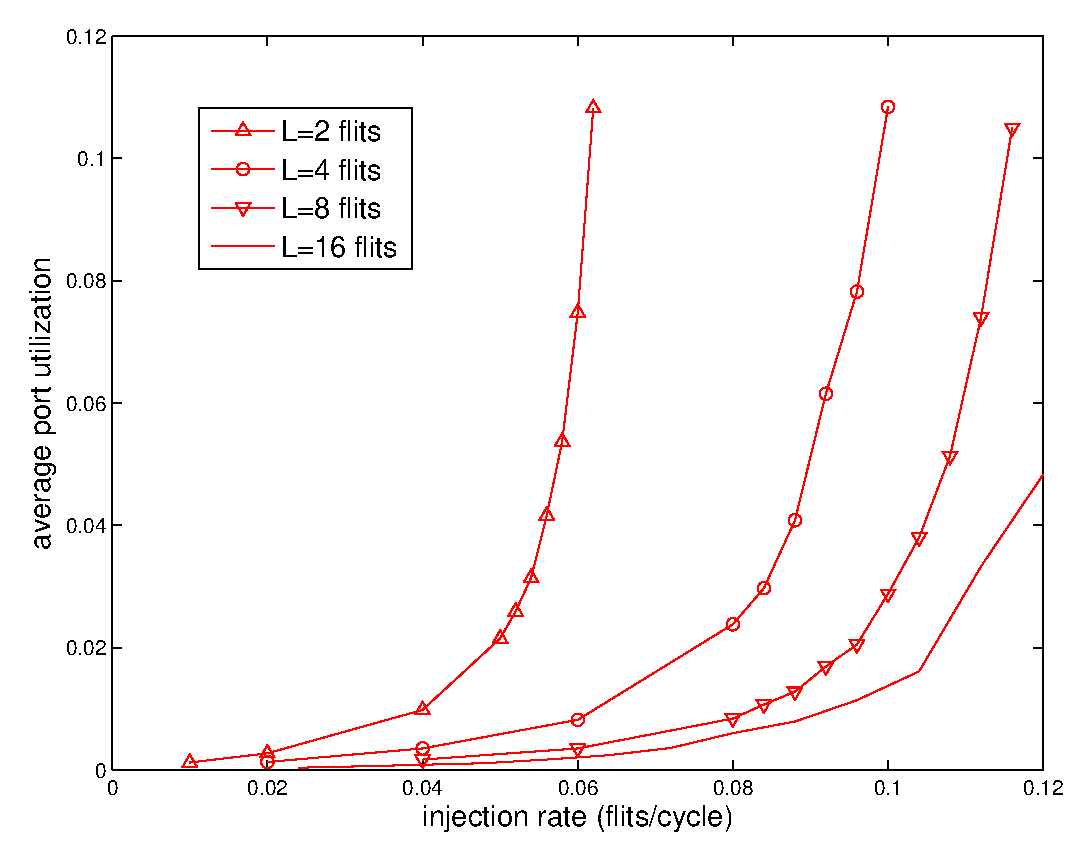
\includegraphics[scale=0.4]{figures/util.eps}
\caption{The port utilization of VC allocator under different injection rate and packet length.}\label{utilization}
\end{figure}

In this paper, we propose an inter-port Adaptive VC Sharing (AVCS) router architecture, which improves network performance and alleviates the blocking caused by both flow control and VC insufficiency by sharing VC and buffer resources among different input ports. Our approach reserves some VC resources for each input port and leaves the other VCs shared by all the input ports. Under low traffic load, the private buffer and VCs are enough to hold all the incoming packets. While under high traffic load, the shared VCs and buffer can be employed to alleviate the blocking caused by both flow control and VC insufficiency. Another contribution of this paper is that we propose the idea of request port sharing to reduce the complexity of VCA and SWA, which multiplexes the request ports of VCA and SWA between shared VCs and private VCs. This scheme allows us to employ small-scale VCA and SWA to arbitrate among large amount of VC request.

The reset of this paper is organized as follows: A summary of related work follows in Section \ref{related}. We introduce the micro-architecture of AVCS in Section \ref{implemented}. Related experimental results are presented in Section \ref{experiemnts}. Finally, we conclude this paper and give the future work in Section \ref{conc}.

\section{Related Work}\label{related}
The input buffer accounts for a large fraction of the overall area and power budget of typical NoC router \cite{1650108}\cite{ChPe03}. Thus, reducing buffer capacity and improving buffer utilization is essential to implement a high-performance NoC router without introducing significant hardware overhead. A proper buffer organization and management scheme is necessary to increase the buffer utilization of wormhole-switched NoC router. There have been significant works focusing on this issue, and several solutions have been proposed.

Virtual Channel Regulator (ViChaR) proposed in \cite{NPKV06} utilizes a table-based Unified Buffer Structure (UBS) to dynamically allocate the buffer slots for each VC according to the traffic condition. Although the buffer utilization and network performance are greatly improved, it introduces significant power burden due to the introduction of additional control logic. The router architecture based on Dynamically Allocated Multiple Queue (DAMQ) \cite{liu2006shared} can provide better performance than typical router while keeping the hardware cost low. To eliminate the additional three-cycle delay of conventional DAMQ structure, a prefetch mechanism was proposed in \cite{6310960}. In \cite{4555894}, the authors proposed a Linked-List based buffer Structure (LLS) and congestion avoidance scheme to improve the network performance and reduce the power and area cost of NoC router. An VC renaming mechanism was proposed in \cite{6296442} to virtualize the physical VC and increase the robustness of NoC router in case of failure. In addition, to alleviate the performance degradation caused by coupling among VCs, an adaptive back-pressure mechanism was proposed in \cite{BeckerJMD12}.

In \cite{Neishaburi:2009:RAN:1531542.1531658}\cite{5770788}, inter-port buffer sharing was proposed to further improve the buffer utilization of typical router. The control logic of this fully shared scheme is more complex than the intro-port buffer sharing schemes, which introduces significant hardware overhead \cite{Park2008}. Accordingly, a similar inter-port buffer-stealing scheme for the wormhole-switched NoC router without VC was proposed in \cite{5722177}. To alleviate the addition control overhead of fine-grained buffer sharing, a Partial Virtual Channel Sharing NoC (PVS-NoC) was proposed in \cite{5739053}, which shares some FIFO buffer between neighbor input port.

The common characteristic of all these proposals is that they reserve large amount of VCs at each port and share buffer resources among VCs to improve buffer utilization and network performance. Whereas, reserving too many VCs introduces significant hardware overhead and makes the utilization of VCA and SWA very low. In addition, under some real-world traffic pattern, the uniformly distributed VC architecture is inefficient because it can not adapt the dynamical change of network traffic. Thus, only combining the buffer sharing and VC sharing can we implement a high-performance NoC router without introducing significant hardware overhead.

\section{Proposed AVCS Router Architecture}\label{implemented}
\subsection{Key Design Consideration}
Virtual channel provides a way to multiplex the physical channel in wormhole-switched NoC to reduce the Head-of-Line (HoL) blocking and deadlock. To avoid packet interleaving, an VC can only be reallocated when the tail flit of previous packet has been completely transmitted to the downstream router. If all the VCs have been occupied, blocking occurs because the packets from upstream router can not find an available VC at downstream router. The degradation caused by VC insufficiency is much serious than that of flow control, especially when the packet size is very large. One solution to this problem is that reserving large amount of VCs for each input port, e.g. \cite{NPKV06}\cite{4555894}\cite{5770788}\cite{Neishaburi:2009:RAN:1531542.1531658}\cite{6310960}. Whereas, it makes the VCA and SWA very complex, and a large amount of registers should be used to track the state of VC resources. Another promising approach is by sharing the buffer and VCs among all the input ports, and allocate buffer and VC resources on demand according to the traffic condition and the VC status of each input port.

While designing the inter-port buffer and VC sharing scheme, the following four issues should be considered:
\begin{enumerate}
\item Interference caused by buffer sharing: When buffer resources are shared among input ports, an adversarial workload injected from one input port might monopolize all the buffer space of the other ports and cause global congestion. Thus, special care should be taken to prevent the blockage from spreading to other ports.
\item Read/Write conflicts caused by buffer sharing: Since each buffer bank can be accessed by multiple input ports, potential conflicts might occur when multiple input ports trying to access the same bank. Thus, additional read/write control logic and scheduling policies should be implemented to avoid hazard.
\item Trade-off between hardware overhead and performance: Although the inter-port buffer sharing can further improve the performance of typical router, it introduces additional hardware overhead. Thus, the trade-off between performance and hardware overhead is necessary to design a high-performance NoC router with acceptable hardware overhead.
\item The complexity of VCA and SWA: When inter-port VC sharing is implemented, the maximal number of VC each input port can use is equal to the total number of private VCs and shared VCs, which is larger than that of typical router. Thus, special care should be taken while designing VCA and SWA, since they occupy large chip area and restrict the frequency of router.
\end{enumerate}

\subsection{Proposed Micro-architecture}
Taking all these aspects into consideration, we proposed the Adaptive VC Sharing (AVCS) NoC router architecture, as shown in Fig. \ref{architecture}. This proposal realizes partial buffer and VC sharing: each input port contributes a small portion of their buffer and VC resources to form shared buffer banks. All these shared buffer banks have an unique bank ID, which can be accessed by all the input ports of a router. For an AVCS router with five input ports, there are five banks in total, and each shared bank manages their own buffer space independently. The owner of each shared buffer bank is determined by their own shared buffer allocator ($\textcircled{4}$ in Fig. \ref{architecture}). The buffer allocator is a Finite State Machine (FSM), which grants a new owner according to the traffic condition of each input port whenever this bank keeps idle for several cycles.
\begin{figure}
  \centering
  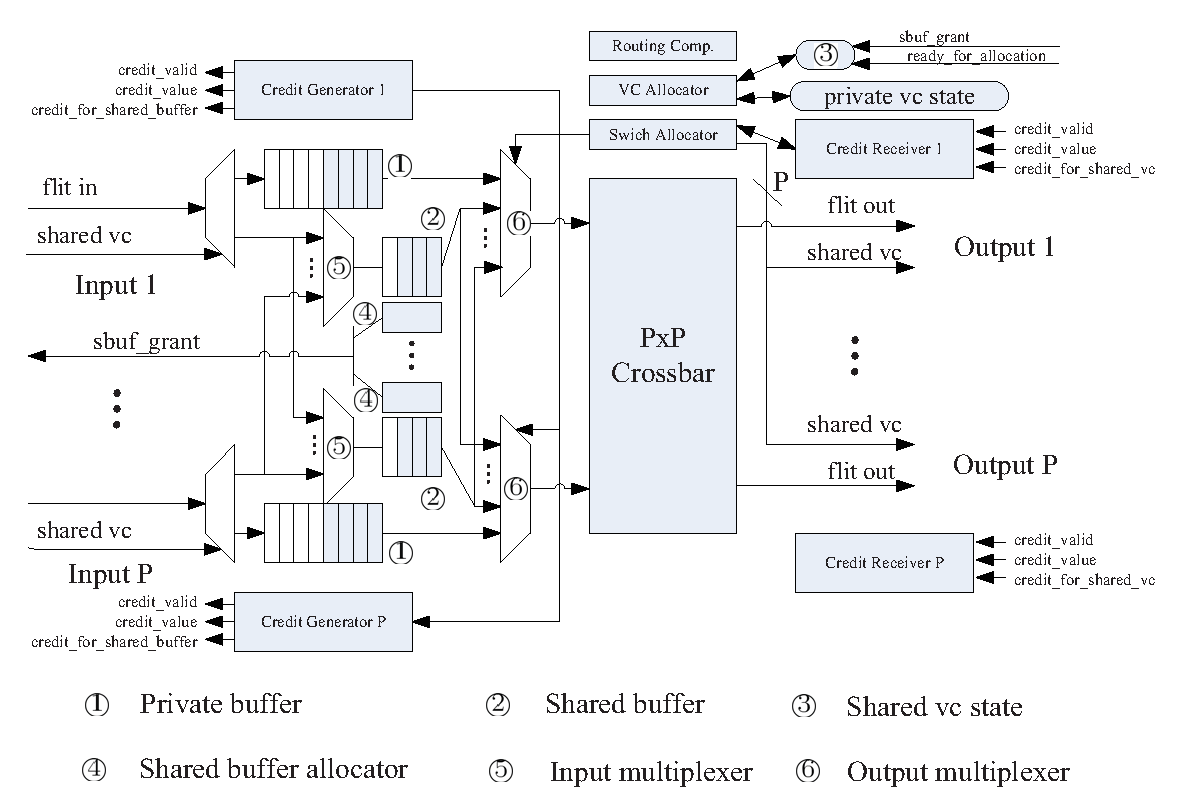
\includegraphics[scale=0.4]{figures/architecture.eps}
  \caption{The proposed AVCS router architecture}\label{architecture}
\end{figure}

After the buffer allocator determines the new owner of shared buffer bank, the allocation results are sent to the upstream routers by raising the \emph{sbuf\_grant} signal. Each output port of neighbor router updates the shared VC state upon receiving the signal. The shared VCs are allocated at the granularity of bank: Only when a shared buffer bank is granted to an input port, the corresponding shared VCs can be utilized by this input port. The SWA schedules the flits located at both shared VCs and private VCs to traverse the crossbar and enter the input port of downstream router. Upon arriving the input port of a router, a flit is written into the shared or private buffer according to the \emph{shared\_vc} signal. Each shared buffer bank utilizes a multiplexer ($\textcircled{5}$ in Fig. \ref{architecture}) controlled by the buffer allocator to select the flits coming from the owner port. Similarly, each input port of the crossbar uses a multiplexer ($\textcircled{6}$ in Fig. \ref{architecture}) controlled by the SWA to select the flits from either private buffer or shared buffers.

The credit-based flow control requires a credit receiving module at the output port of upstream router and a credit generating module at the input port of downstream router. Since the private buffer and shared buffer are managed independently in AVCS router, a dedicated credit counter for each shared buffer bank is necessary. To distinguish whether the credit is for the shared VCs, an additional signal \emph{credit\_for\_shared\_vc} driven by credit generator is connected to the corresponding credit receiver besides the \emph{credit\_valid} and \emph{credit\_value} signal, as shown in Fig. \ref{architecture}.

To improve the performance with limited buffer resources, we must manage and allocate the buffer resources dynamically according to the traffic condition. Two methods have been proposed to achieve this aim, e.g. UBS \cite{NPKV06}\cite{5770788} and LLS \cite{4555894}\cite{Neishaburi:2009:RAN:1531542.1531658}. Since UBS is only applicable to the fixed-length packet network, we adapt LLB scheme for both shared and private buffer in our approach to increase the buffer utilization. Five tables are necessary to implement LLB scheme, as shown in Fig. \ref{linklist}. A Next Pointers Table records the next slot address for each buffer slot; A Tail Pointers Table maintains the writing address of each VC; A Header Pointers Table keeps the reading address for each VC; A Free Slots Table tracks the address of all the unused buffer slot; In addition, a VC State Table is used to identify the occupied VCs.
\begin{figure}
  \centering
  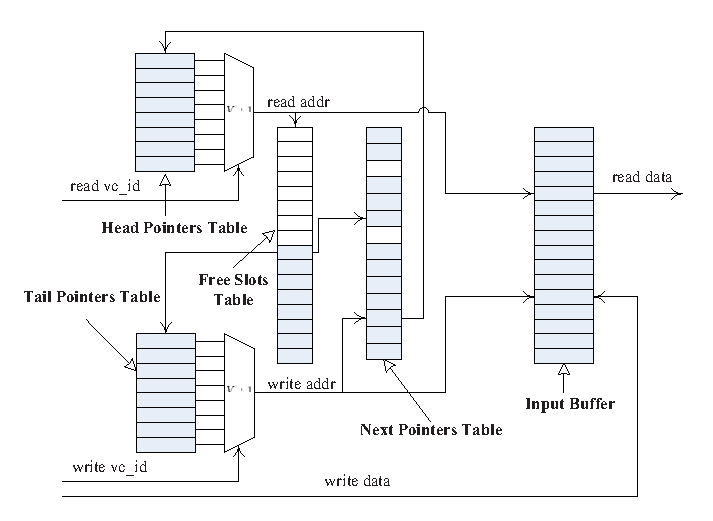
\includegraphics[scale=0.6]{figures/linklist.eps}
  \caption{The internal structure of shared/private buffer}\label{linklist}
\end{figure}

The main difference between typical router and our proposal lies in the buffer and VC organization, as shown in Fig. \ref{org}. For the same amount of buffer slots $B$ and VC number $V$, each input port of our AVCS router reserves $5/6B$ slots as private buffer and shares $B/6$ slots with other input ports. Meanwhile, the VC resources within the shared buffer bank are shared among all these input ports. The shared buffer can change their owner according to the traffic condition of each input port to improve the buffer utilization and network performance. Under low traffic load, the private buffer and VC resources of each input port is capable of delivering all the incoming traffic. While under high traffic load, the shared buffer and VCs of idle input ports will be designated to the congested port later to alleviate the congestion. The amount of buffer slots each input port can use lies between $5/6B$ and $10/6B$, in contrast to $B$ of typical router. Similarly, the number of VCs each input port can use lies between $5/6V$ and $10/6V$.
\begin{figure}[h]
  \centering
  \subfloat[AVCS-NoC]{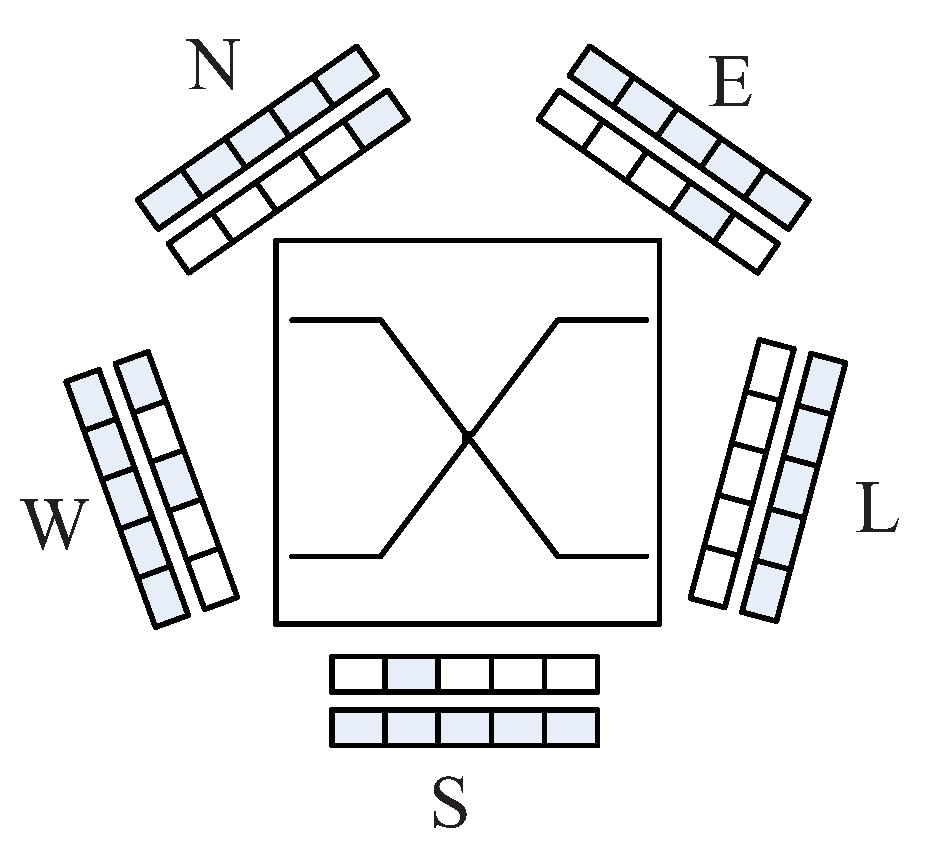
\includegraphics[scale=0.25]{figures/avcsbuf.eps}\label{avcsbuf}}\hspace{10pt}
  \subfloat[typical router]{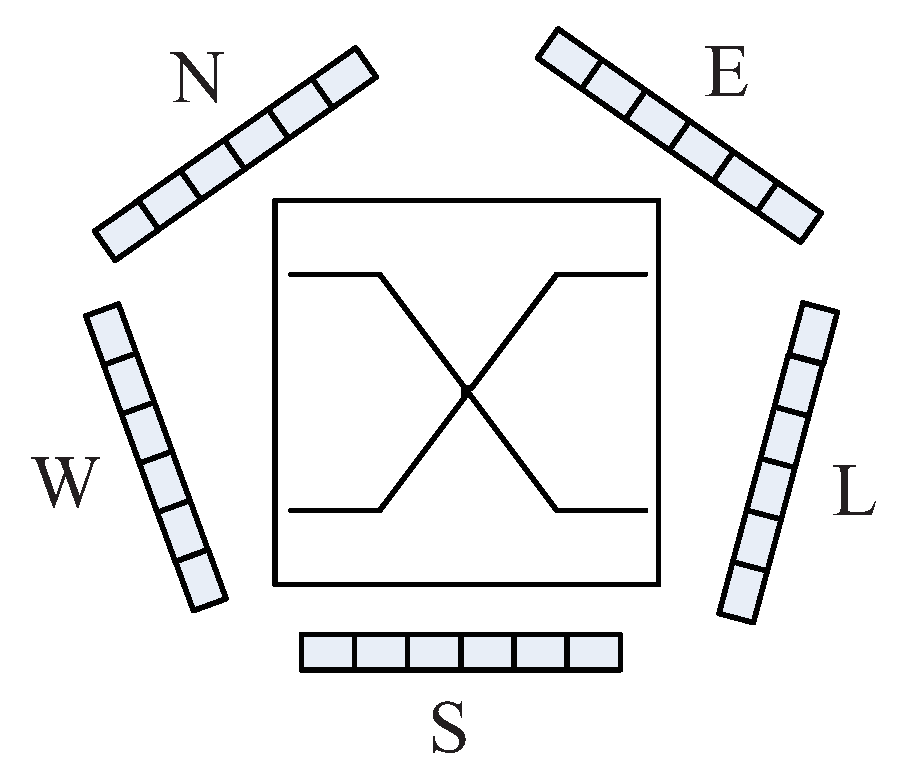
\includegraphics[scale=0.25]{figures/typicalbuf.eps}\label{typicalbuf}}
  \caption{Buffer organization of AVCS-NoC and typical router.}\label{org}
\end{figure}

Our proposal resolves all the aforementioned issues:
\begin{enumerate}
\item This architecture is a partial buffer and VC sharing scheme, even when all the shared buffer is occupied by some input ports, the other ports can still use their private buffer to guarantee the transmission of packets, which alleviates the interference caused by complete inter-port buffer and VC sharing.
\item The hardware overhead of our proposal is much lower than the fully-shared scheme, e.g. \cite{Neishaburi:2009:RAN:1531542.1531658}\cite{5770788}, which realizes better trade-off between cost and performance. We will discuss this issue in subsection \ref{controllogic}.
\item The shared buffer is divided into several small banks to support parallel access. Each bank can only be granted to one input port at any time, which avoid the multiple read/write conflicts.
\item In order to minimize the complexity and hardware cost of VCA and SWA, we let the shared VCs and private VCs sharing the same request port, as explained in subsection \ref{allocmux}. This approach makes it possible to arbitrate large amount of VCs by using a smaller VCA and SWA, which reduces the complexity of these two allocators significantly.
\end{enumerate}

The AVCS router architecture is different from the previously proposed ViChaR \cite{NPKV06}, which needs fully re-implement the router pipeline. In contrast, our approach augments typical router architecture \cite{DaTo01} by adding a shared buffer allocator for each shared buffer bank and re-implementing VCA and SWA. The buffer allocator works in parallel with router pipeline, which imposes no negative effect on the critical path of entire router. We will introduce the implementation of buffer allocator, VCA and SWA in the following two subsections.

\subsection{Shared Buffer Allocation Module}\label{bufmanage}
The shared buffer allocator in our AVCS router is an FSM, which has three states: Enable\_Allocation(EA), Disable\_Allocation(DA) and Change\_Allocation(CA), as shown in Fig. \ref{allocFSM}. The \emph{ready\_for\_allocation} signal keeps on valid while in Enable\_Allocation state. In this state, the shared buffer and VCs can be used by the input port indicated by the \emph{sbuf\_grant} signal. We say that a shared buffer bank is idle when it is empty and no output VC of upstream router was designated to it. When the shared buffer bank keeps on idle for $K$ cycles, we can infer that this input port does not need this bank temporally. Thus, we can reallocate it to other input ports which require more buffer and VC resources. The threshold $K$ is a design parameter, which affects the allocation results and the performance of entire network. For a real-world application, the optimal $K$ can be chosen by experiments. To avoid the shared buffer is reallocated while changing status, the FSM first enters the Disable\_Allocation state. At this state, the \emph{ready\_for\_allocation} signal goes down to disable the output VC allocation at upstream router. When the shared buffer bank is empty and no shared VCs on this bank are allocated, the FSM enters the Change\_Allocation state. At this state, the buffer allocator chooses the new owner for the shared buffer according to the congestion status of each input port and the current owner of this bank (indicated by \emph{sbuf\_grant}), as described in Alg. \ref{alg:bufferalloc}. Then, the FSM enters Enable\_Allocation state and begins another allocation period.
\begin{figure}[htb]
  \begin{minipage}[b]{0.3\textwidth}
    \centering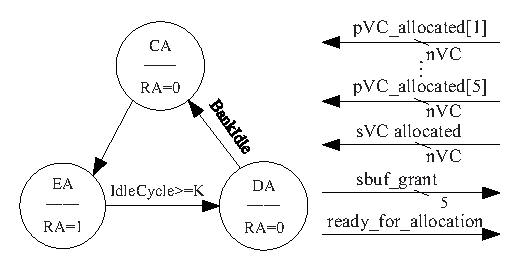
\includegraphics[scale=0.52]{figures/allocFSM.eps}
    \caption{The FSM of buffer allocator}\label{allocFSM}
  \end{minipage}%
  \begin{minipage}[b]{0.2\textwidth}
    \centering
    \begin{tabular}{|c|c|}
      \hline
      Port & Encode \\
      \hline\hline
      East  & 10000 \\
      \hline
      West    & 01000 \\
      \hline
      South &   00100\\
      \hline
      North & 00010\\
      \hline
      Local & 00001\\
      \hline
    \end{tabular}
    \caption{Port Encoding}\label{portencode}
  \end{minipage}
\end{figure}

To simplify the allocation algorithm, we choose the owner of each shared buffer bank in round-robin order. This is achieved by using a five-bit register \emph{port\_mask} to filter out the ports can not be chosen as candidate at current allocation period (Step 4 and Step 7). Initially, these five buffer banks belongs to different input ports (Step 3 and Step 6). When the FSM enters Change\_Allocation state, the five-bit \emph{port\_busy} (generated in Step 11) and \emph{port\_mask} registers are used to determine the new owner of this bank (Step 13 to 21). The fundamental idea of this algorithm is that choosing the candidate in order and skip the idle input ports to accelerate this process. If the position of the left-most `1' in the selector signal (generated at Step 13) matches one of the input ports listed in Fig. \ref{portencode}, the shared buffer is granted to this port. The encoding scheme also indicates that the choosing order of this algorithm is: East $\to$ West $\to$ South $\to$ North $\to$ Local $\to$ East. One example of how this algorithm functions is illustrated in Fig. \ref{Algorithm}. For a real-world application, we can also change the allocation algorithm to adapt the characteristic of traffic pattern.
\begin{algorithm}[h]
\caption{Shared buffer allocation}\label{alg:bufferalloc}
\begin{algorithmic}[1]
\STATE \textbf{Initialized:}
\STATE \ \ \ \ \textbf{if}(bank\_id==5)
\STATE \ \ \ \ \ sbuf\_grant = 5'b00001;
\STATE \ \ \ \ \ port\_mask = 5'b11111;
\STATE \ \ \ \ \textbf{else}
\STATE \ \ \ \ \ sbuf\_grant = East $>>$ bank\_id;
\STATE \ \ \ \ \ port\_mask = 5'b11111 $>>$ (bank\_id+1);
\STATE \ \ \ \ \textbf{endif}
\STATE \textbf{Change\_Allocation:}
\STATE \ \ \ \ \textbf{for}(p=1;p$<=$5;p=p+1)
\STATE \ \ \ \ \ port\_busy[p] = $|$ pVC\_allocated[p];
\STATE \ \ \ \ \textbf{endfor}
\STATE \ \ \ \ selector = port\_mask \& port\_busy;
\STATE \ \ \ \ \textbf{case}(selector)
\STATE \ \ \ \ \ \ \ \ 5'b1xxxx: sbuf\_grant = East; port\_mask=5'b01111;
\STATE \ \ \ \ \ \ \ \ 5'b01xxx: sbuf\_grant = West; port\_mask=5'b00111;
\STATE \ \ \ \ \ \ \ \ 5'b001xx: sbuf\_grant = South; port\_mask=5'b00011;
\STATE \ \ \ \ \ \ \ \ 5'b0001x: sbuf\_grant = North; port\_mask=5'b00001;
\STATE \ \ \ \ \ \ \ \ 5'b00001: sbuf\_grant = Local; port\_mask=5'b11111;
\STATE \ \ \ \ \ \ \ \ default: port\_mask=5'b11111;
\STATE \ \ \ \ \textbf{endcase}
\end{algorithmic}
\end{algorithm}
\begin{figure}[h]
\centering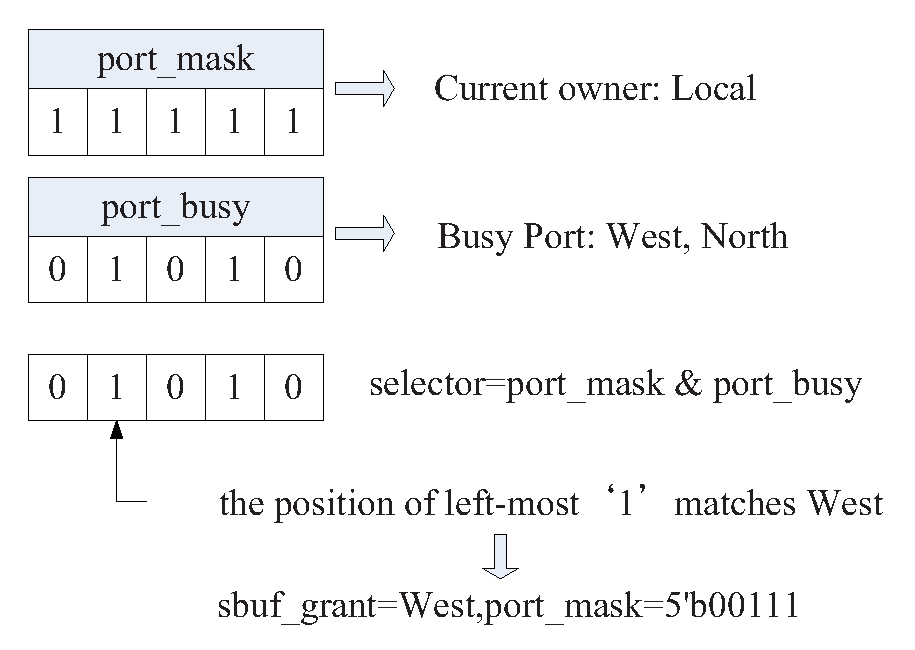
\includegraphics[scale=0.5]{figures/Algorithm.eps}
\caption{Step-by-step example of buffer allocation algorithm}\label{Algorithm}
\end{figure}

\subsection{VC and SW Allocator}\label{allocmux}
The goal of inter-port buffer and VC sharing is to alleviate the performance degradation caused by flow control and VC blocking. Because the allocation results changes with traffic load, our architecture is more suitable to address the blocking caused by unbalanced VC and buffer requirement of different input ports. The VCs each input port can use in AVCS router includes the private VCs owned by this port and the VCs shared among all the ports. Thus, the number of VCs each input port can use varies with traffic condition, since an input port with heavy traffic load is likely to own more shared buffer banks. Denote the number of input ports and the maximal shared VCs (including private and shared VCs) each input port can use as $P$ and $V_{max}$. The VCA matches $P\times V_{max}$ requests from $P$ input ports with $P\times V_{max}$ output VCs. Similarly, the SWA matches the $P\times V_{max}$ request from $P$ input ports to $P$ output ports. To support the worst-case VC and switch allocation, one solution is that by adapting a $PV_{max}\times PV_{max}$ VCA and a $PV_{max}\times P$ SWA. However, this makes these two allocators complex and introduce significant hardware overhead.

In this paper, we employ another approach. Our approach lies on two properties of AVCS router: (1) The maximum number of shared VCs in AVCS-NoC is equal to the number of private VCs owned by each input port, and (2) the minimum number of shared VCs each input port can use is zero. Thus, the actually available VCs of each input port can use lies between $1/2V_{max}$ and $V_{max}$. We assign an unique ID to each shared VC, and let these shared VCs compete for the request ports with private VCs. Then, we can use a $1/2PV_{max}\times 1/2PV_{max}$ VCA and a $1/2PV_{max}\times P$ SWA to perform the VC and switch allocation. The reason we employ a smaller VCA and SWA with port sharing rather than a larger allocator lies in the fact that the port utilization of VCA and SWA is very poor, especially for the VCA, as demonstrated in Fig. \ref{utilization}. This is because only the head flit of a packet can issue an VC allocation request and the corresponding request port will keep on idle until the tail flit departure from this VC. The idle request port can be reused to improve the utilization.

Specifically, when a shared buffer is designated to an input port, the \emph{elig\_svc} flags of all the corresponding shared VCs are asserted to allow the granting of a request. To enable the sharing of request port, we add a $2:1$ selector to each request port to choose a request from either private VC or shared VC, as shown in Fig. \ref{vcallocator}. This selector chooses these two input VCs in round-robin order to prevent livelock. Then a $1/2PV_{max}\times 1/2PV_{max}$ separable input-first allocator \cite{DaTo04} is used to perform the subsequent arbitration. The separable input-first allocator employs $1/2V_{max}$ $1/2V_{max}:1$ arbiters at each input port to grant at most 1 output VC to this request port, and each output port uses $1/2V_{max}$ $1/2PV_{max}:1$ arbiters to select one input request for each output VC. In order to make the allocation of shared buffer sensitive to the dynamical change of traffic, we assign lower priority to the shared output VC. A shared output VC is allocated only when all the private VCs have been occupied. In contrast, to meet the same arbitration demand, the separable input-first allocator used in the typical router needs $V_{max}$ $V_{max}:1$ arbiters to guarantee each input VC can only request at most 1 output VC, and each output port employs $V_{max}$ $PV_{max}:1$ arbiters to grant each output VC to an unique input VC.
\begin{figure}[h]
\centering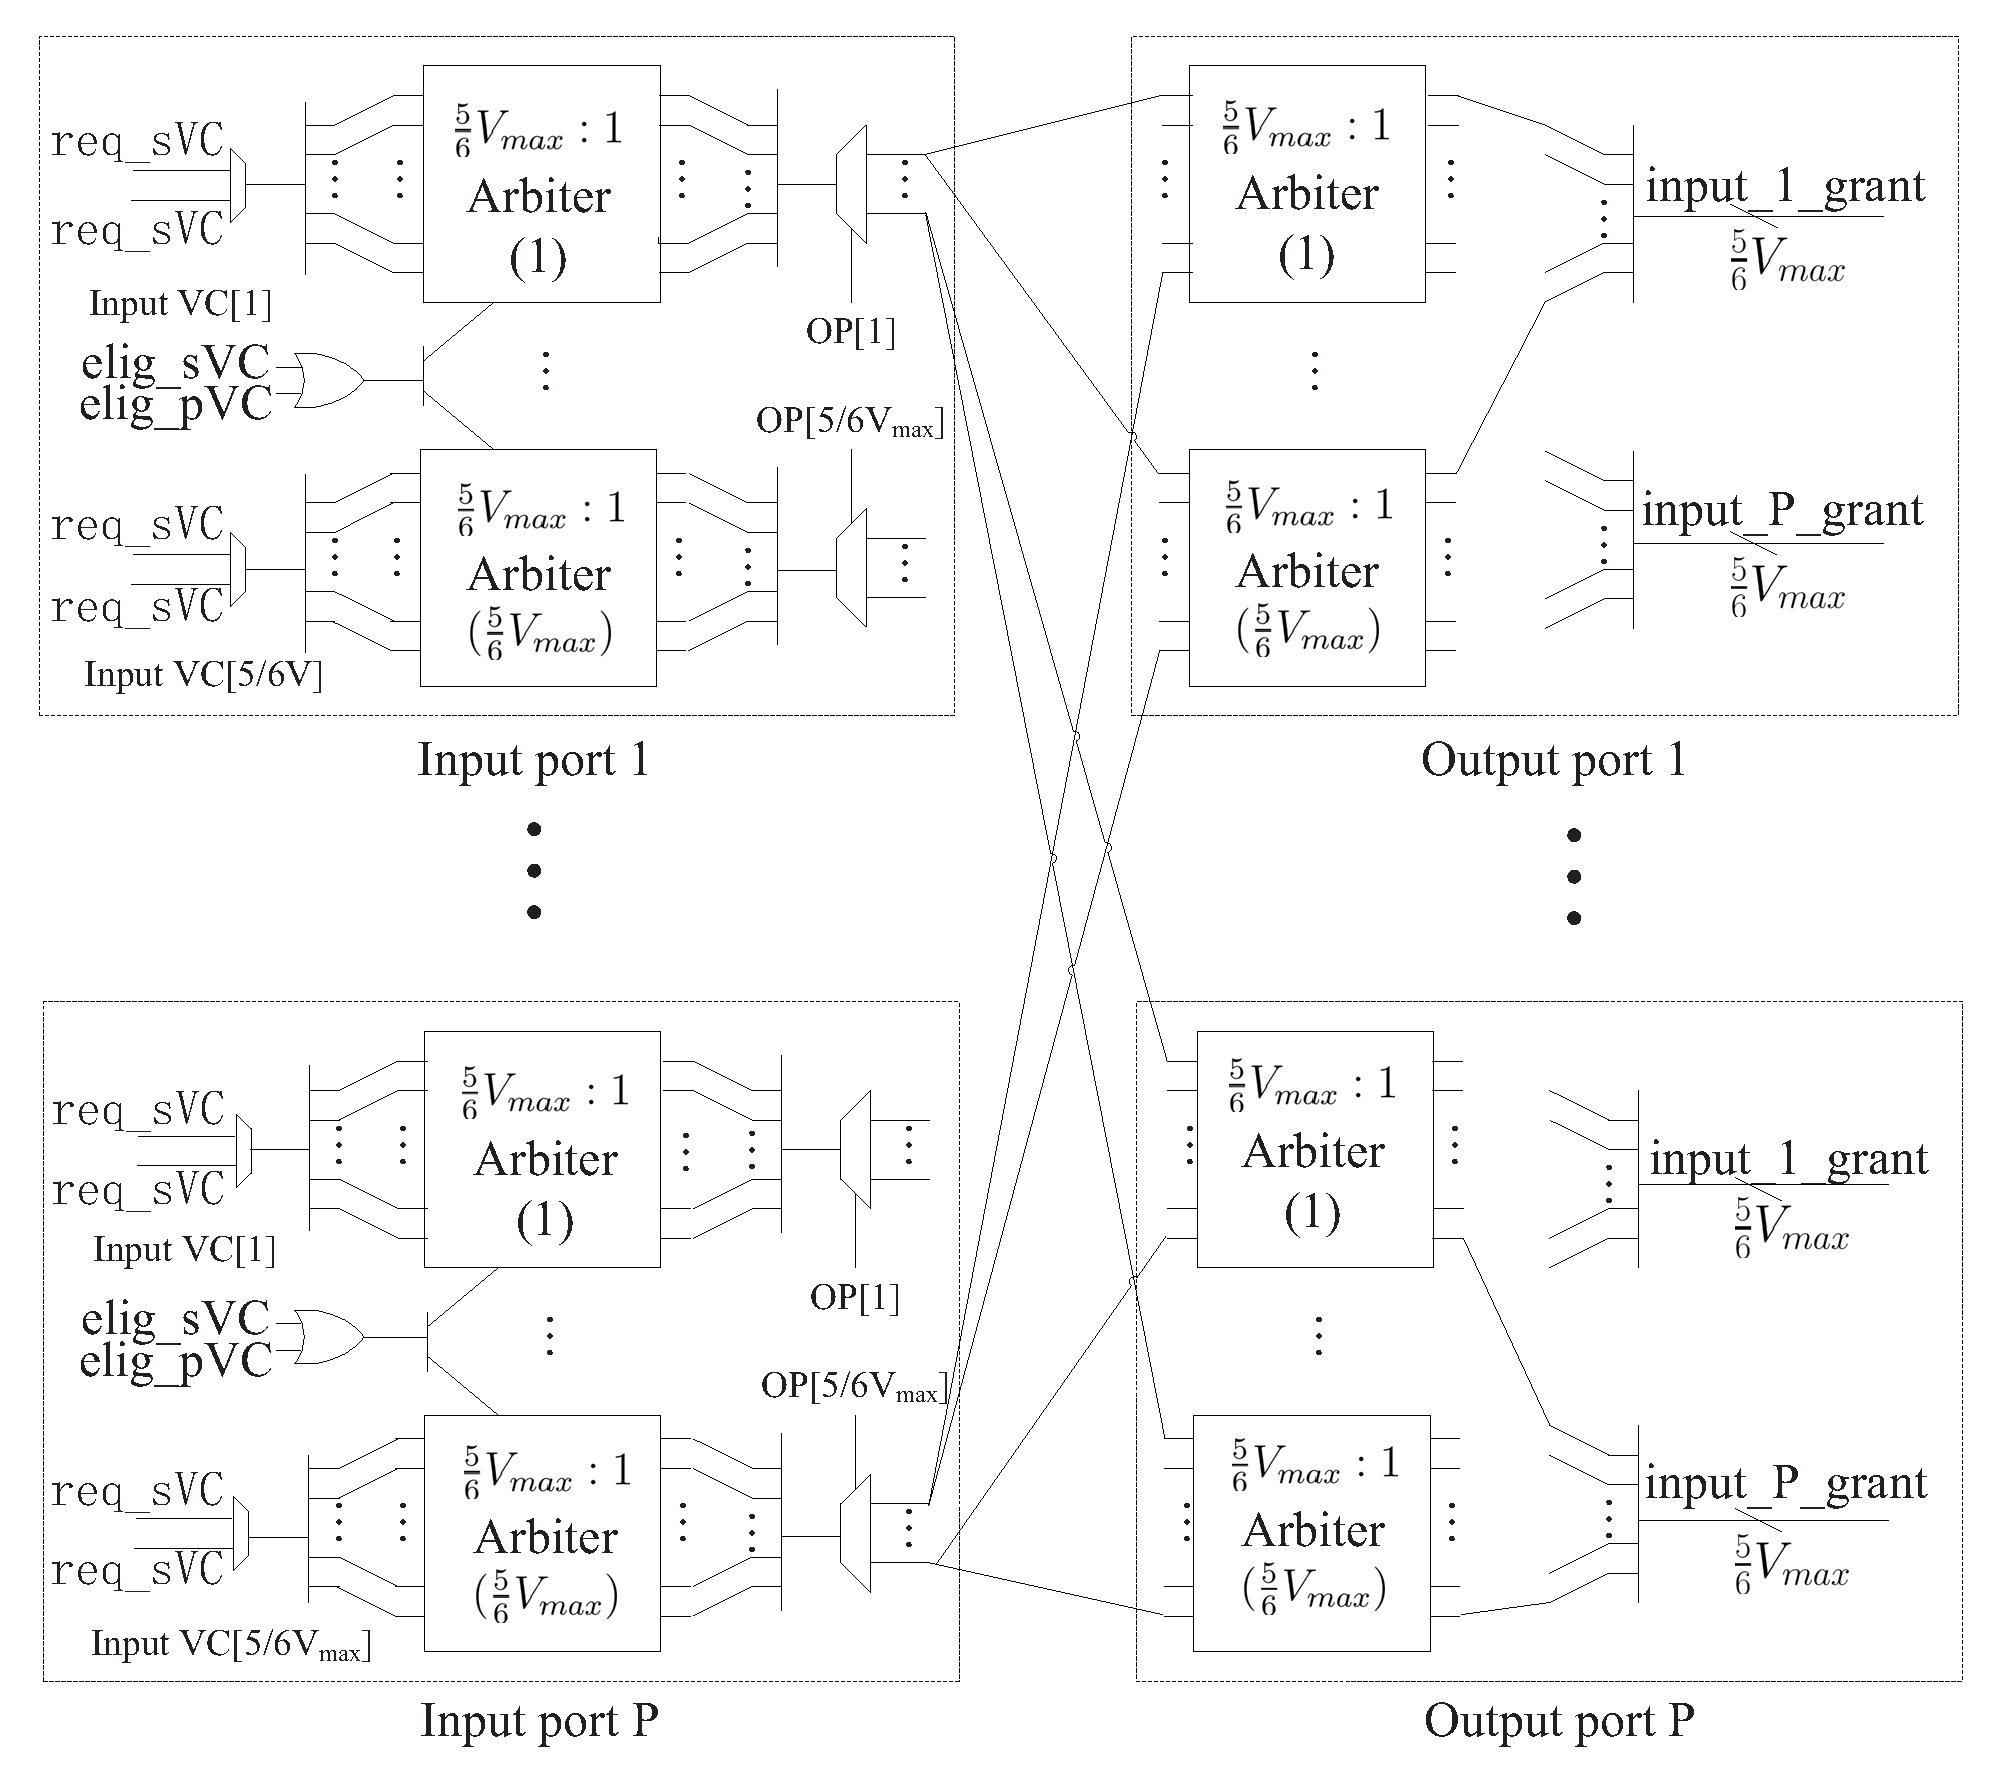
\includegraphics[scale=0.25]{figures/vcalloc.eps}
\caption{The Implementation of VCA}\label{vcallocator}
\end{figure}

Similarly, for the SWA, if one of the VC is blocked due to some reasons, the corresponding request port can be reused by the shared VC. As shown in Fig. \ref{swallocator}, we first use a $2:1$ arbiter to select on request from either shared VC or private VC at the first stage. The selection is performed in round-robin order to avoid livelock. The second stage utilizes a $1/2V_{max}:1$ arbiter at each input port to select one winner from all the request. Then, a third stage with a $P:1$ arbiter at each output port is applied to select one request for each output. In contrast, to meet the same arbitration demand, the separable input-first allocator used in typical router needs $V_{max}$ $V_{max}:1$ arbiters to guarantee at most 1 input VC be granted, and each output port employs a $P:1$ arbiters to grant to a unique input VC. We will demonstrate the hardware saving of our proposal in subsection \ref{area}.
\begin{figure}[h]
\centering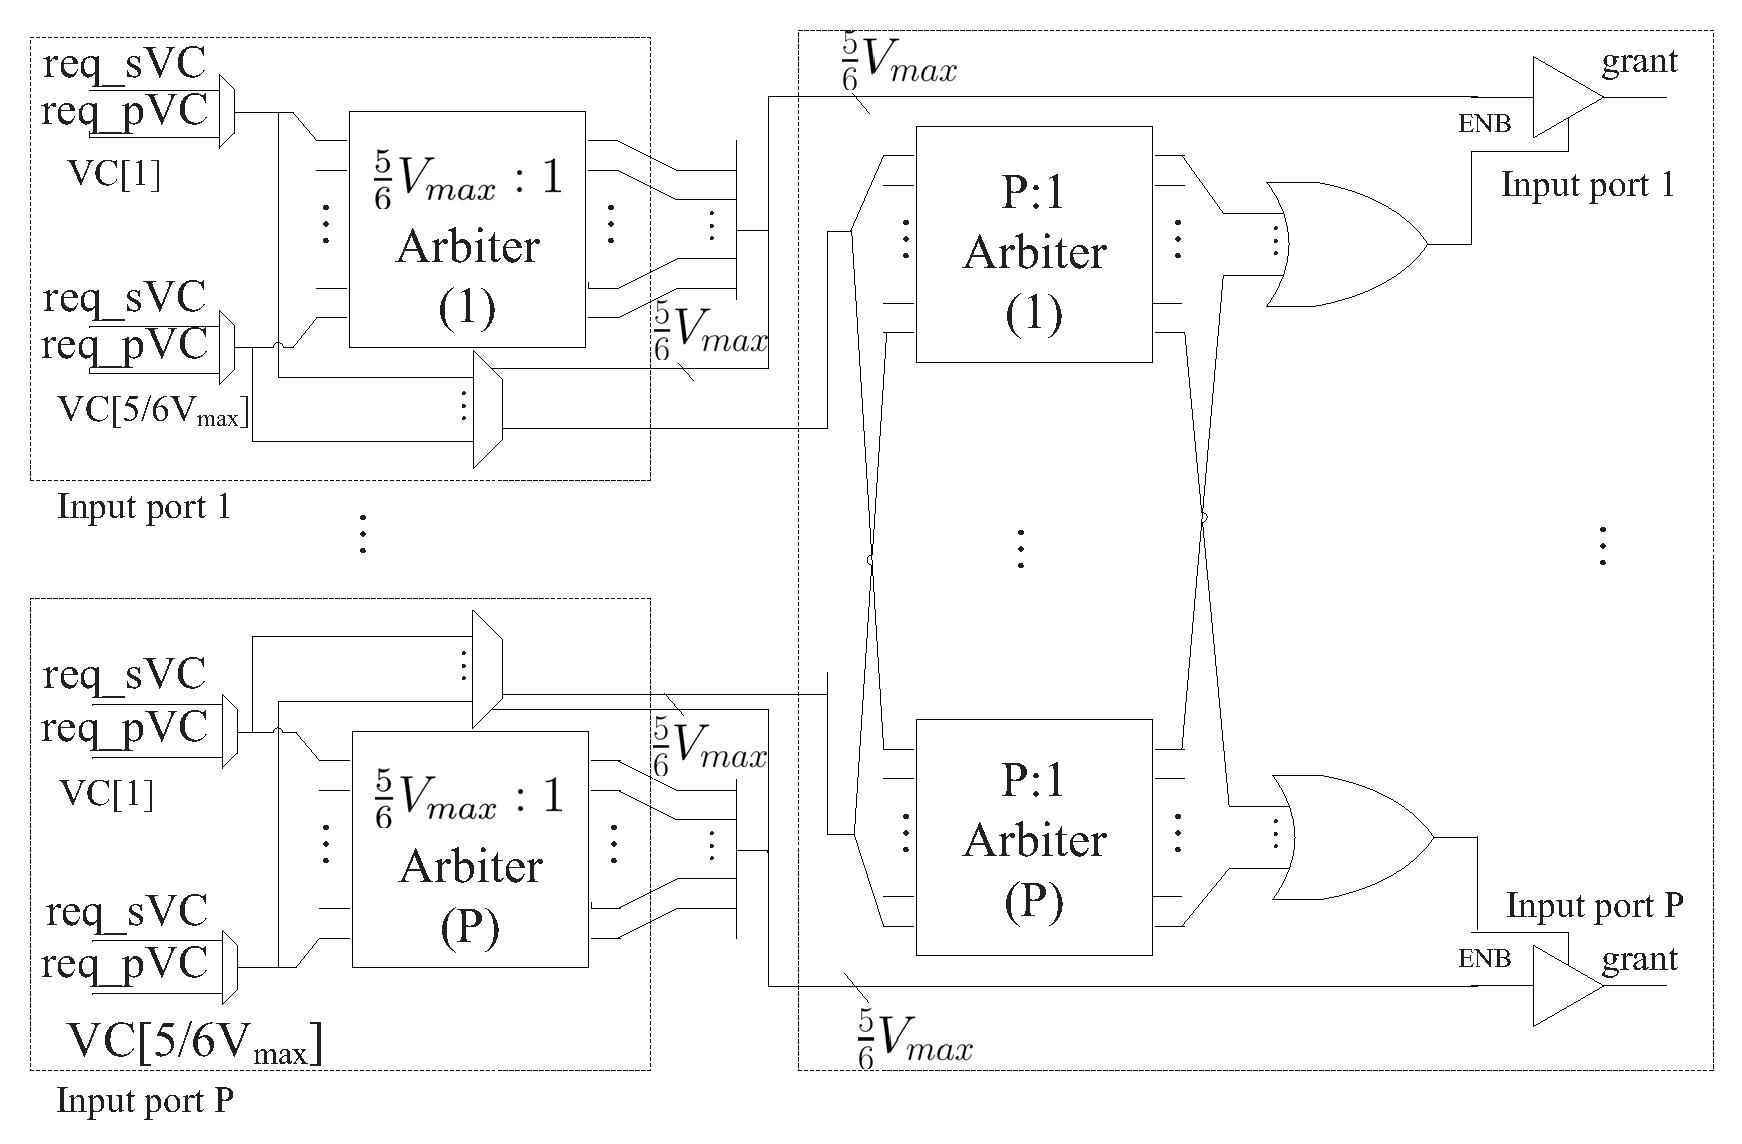
\includegraphics[scale=0.29]{figures/swalloc.eps}
\caption{The Implementation of SWA}\label{swallocator}
\end{figure}

\section{Experimental results}\label{experiemnts}
To compare the performance and hardware overhead of our approach with existing proposals, we implement AVCS router, typical router \cite{DaTo01} and dynamical buffer management router \cite{NPKV06}\cite{4555894} in Verilog HDL. The comparison results on hardware overhead, network performance, power and chip area are presented in the following three subsections.

\subsection{Control Overhead Comparison}\label{controllogic}
Both UBS \cite{NPKV06}\cite{5770788} and LLB \cite{4555894}\cite{Neishaburi:2009:RAN:1531542.1531658} require large amount of control logic to keep track of buffer usage. For the inter-port buffer sharing scheme \cite{Neishaburi:2009:RAN:1531542.1531658}, the hardware overhead is much higher than the intra-port sharing scheme since the Next Pointer and Free Slot Pointer for each input port, the Header Pointer and Tail Pointer for each VC must be able to index all the buffer slot within a router. Supposing dynamical buffer management router \cite{NPKV06}\cite{4555894}\cite{Neishaburi:2009:RAN:1531542.1531658}\cite{5770788} has $B$ buffer slots and $V$ VCs at each input port. Then, our approach has $5/6V$ private VCs and $5/6B$ buffer slots at each input port, and each shared buffer bank has $1/6B$ buffer slots and $1/6V$ shared VCs. For each input port of UBS router, denote by $L$ the packet length. Under the same condition, the VC Availability Tracker and Slots Availability Tracker require $V+\lceil log_2 V\rceil$ and $B+\lceil log_2B\rceil$ registers, respectively; The VC Control Table needs $VL\lceil log_2B\rceil$ registers; Both the Arriving and Departing Flit Pointers require $2V\lceil log_2 L\rceil$ registers. For each input port of LLB router, the Free Slots Table requires $B$ registers to track the unused slots and $\lceil \log_2 B\rceil$ registers to point to the first available slot; The Next Pointers Table requires $B\times \lceil log_2 B\rceil$ registers to maintain the flits order of all the VCs; Both the Head Pointers Table and Tail Pointers Table need $V\times \lceil log_2 B\rceil$ registers. Similarly, the hardware overhead of AVCS can be derived, as shown in Table \ref{control}.
\begin{table}
\caption{Hardware overhead comparison}\label{control}
\centering\begin{tabular}{c|c}
\hline
\hline
Structure & Control Register\\
\hline
UBS \cite{NPKV06}  &   $5((V+B)+(1+LV)\lceil log_2B\rceil+\lceil log_2V\rceil+2V\lceil log_2L\rceil)$\\
\hline
LLB \cite{4555894} & $5(B+(1+B+2V) \lceil log_2B\rceil)$\\
\hline
AVCS    & $5(B+(1+\frac{5}{6}B+\frac{10}{6}V)\lceil log_2\frac{5}{6}B\rceil +(1+\frac{B}{6}+\frac{2}{6}V)\lceil log_2\frac{B}{6}\rceil)$\\
\hline
\end{tabular}
\end{table}

To make concrete comparison, for the same packet length $L=8$ flits, we plot the hardware overhead of each scheme under different VC number and buffer capacity in Fig. \ref{bufcmp1} and Fig. \ref{bufcmp2}. As shown in these two figures, our approach uses the lest control logic, because we divide the buffer resources into several banks, and each bank manages their own buffer resource independently. The total hardware overhead is greatly reduced since the addressing space of each buffer bank is smaller than the other two approaches. When the flit width, VC number, buffer size, packet length are 128bits, 12, 24 flits, 8 flits, respectively, the total hardware overhead of our approach is only 5.37\%, in contrast with 7.16\% and 16.24\% of LLB and UBS approach, respectively. We also need to emphasize that although our proposal introduces additional hardware overhead, the utilization improvement makes it possible to halve the buffer slots without degrading the performance, as presented in the following subsection. Thus, our proposal is cost-efficient.
\begin{figure}[h]
  \centering
  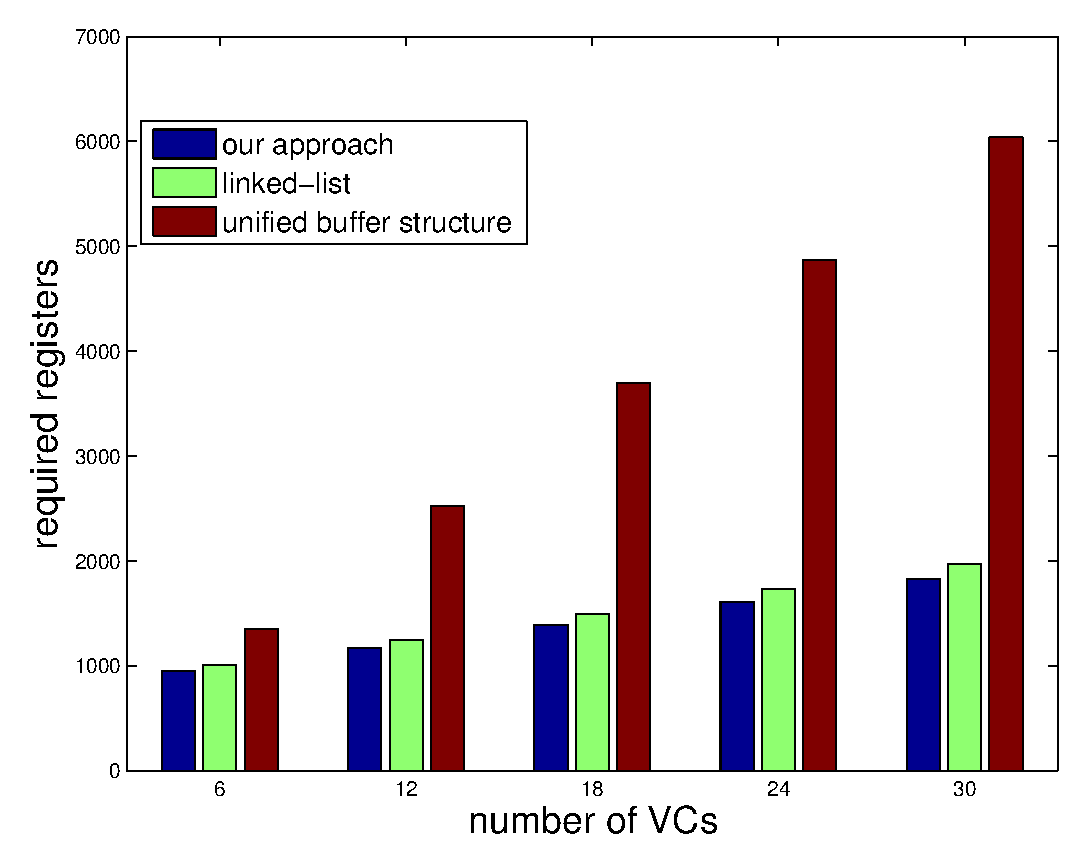
\includegraphics[scale=0.45]{figures/bufcmp1.eps}
  \caption{Hardware Overhead Comparison}\label{bufcmp1}
\end{figure}
\begin{figure}[h]
  \centering
  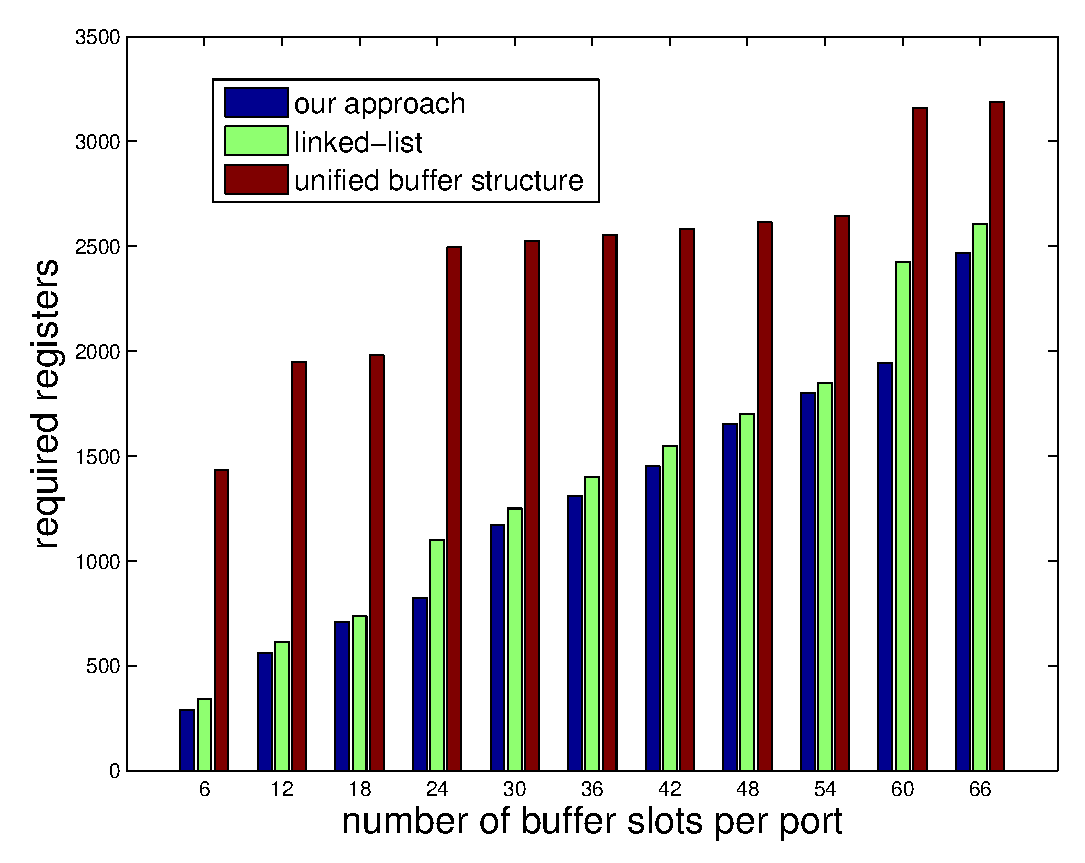
\includegraphics[scale=0.45]{figures/bufcmp2.eps}
  \caption{Hardware Overhead Comparison}\label{bufcmp2}
\end{figure}

\subsection{Performance Comparison}
In this subsection, we compare the performance of AVCS router with typical router \cite{DaTo01} and dynamical buffer management router \cite{NPKV06}\cite{4555894} under synthesis traffic pattern and realistic traffic pattern.
\subsubsection{Synthesis Traffic}
Hotspot and uniform traffic pattern are taken as examples to demonstrate the performance improvement of our proposal over the other two kinds of architectures. The configuration used in our experiment are presented in Table \ref{config}.
\begin{table}[htbp]
\centering
\caption{\label{arcpara}Configuration used in the experiments}\label{config}
\begin{tabular}{|c|c||c|c|}
\hline
topology    & $4\times 4$ mesh  &   routing algorithm & DOR\\
\hline
flit width   & 256 bits & warmup period &   $1\times 10^4$ cycles\\
\hline
packet length & 8 flits & sampling period &   $1\times 10^6$ cycles\\
\hline
\end{tabular}
\end{table}

For typical router architecture, two configurations, i.e. Gen(8,24) and Gen(8,48), are used in our comparison according to their VC number and buffer capacity. The dynamical buffer management router architecture is deployed with 12 VCs and 24 buffer slots per input port, denoted as DBM(12,24). To make a fair comparison, we let each input port of our AVCS router have 20 buffer slots and 10 VCs. The shared buffer have 20 buffer slots and 10 VCs in total, organized as five banks. In this experiment, we set the threshold $K=10$.

As shown in Fig. \ref{hotspotlat}, we find that our approach improves the performance of typical router and dynamical buffer management router under hotspot traffic significantly, take the injection rate 0.00656 flits/node/cycle as an example, our router reduces the average latency over DBM(12,24), Gen(8,24) and Gen(8,48) by 30.1\%, 61.3\% and 29.6\%, respectively. For the uniform traffic, our approach achieves the similar performance as DBM(12,24) and Gen(8,48), but improves the performance of Gen(8,24) significantly, as shown in Fig. \ref{randomlat}. Our AVCS router does not achieve too much gain while comparing with dynamical buffer management router because the congestion status of each input port under uniform traffic pattern is similar.
\begin{figure}[h]
  \centering
  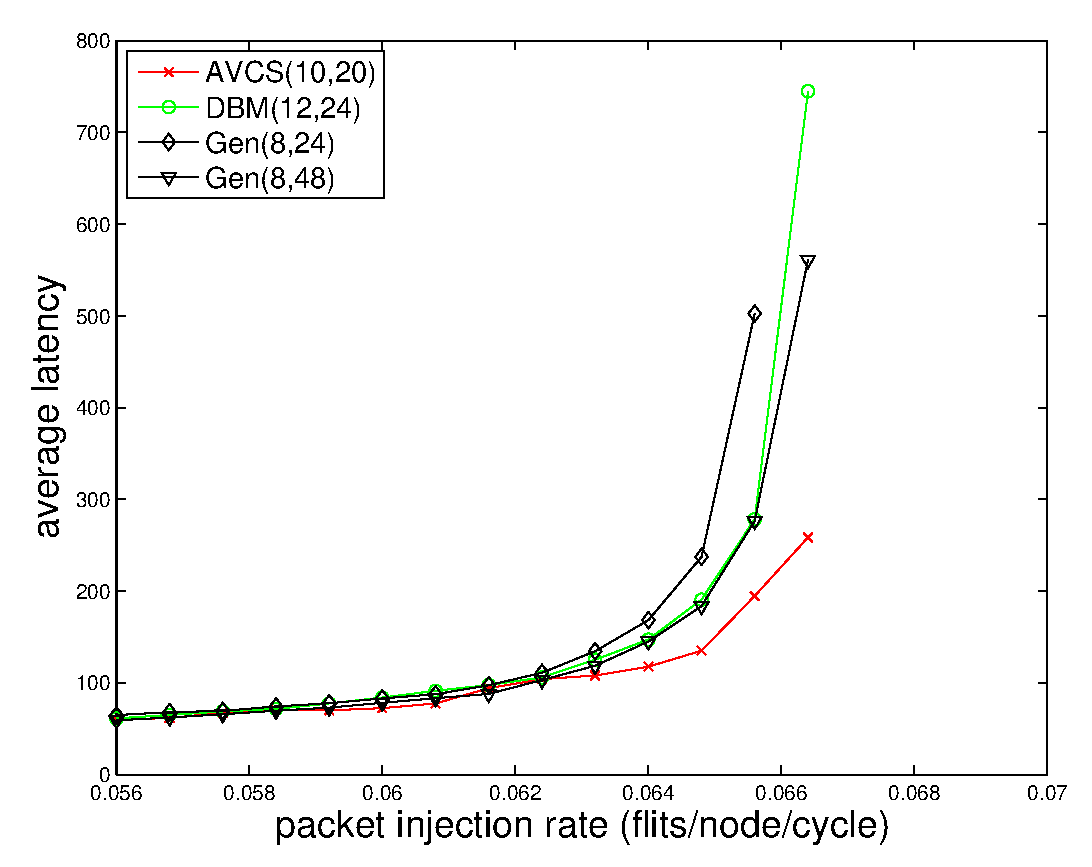
\includegraphics[scale=0.4]{figures/hotspotlat.eps}
  \caption{Latency comparison under hotspot traffic pattern}\label{hotspotlat}
\end{figure}
\begin{figure}[h]
  \centering
  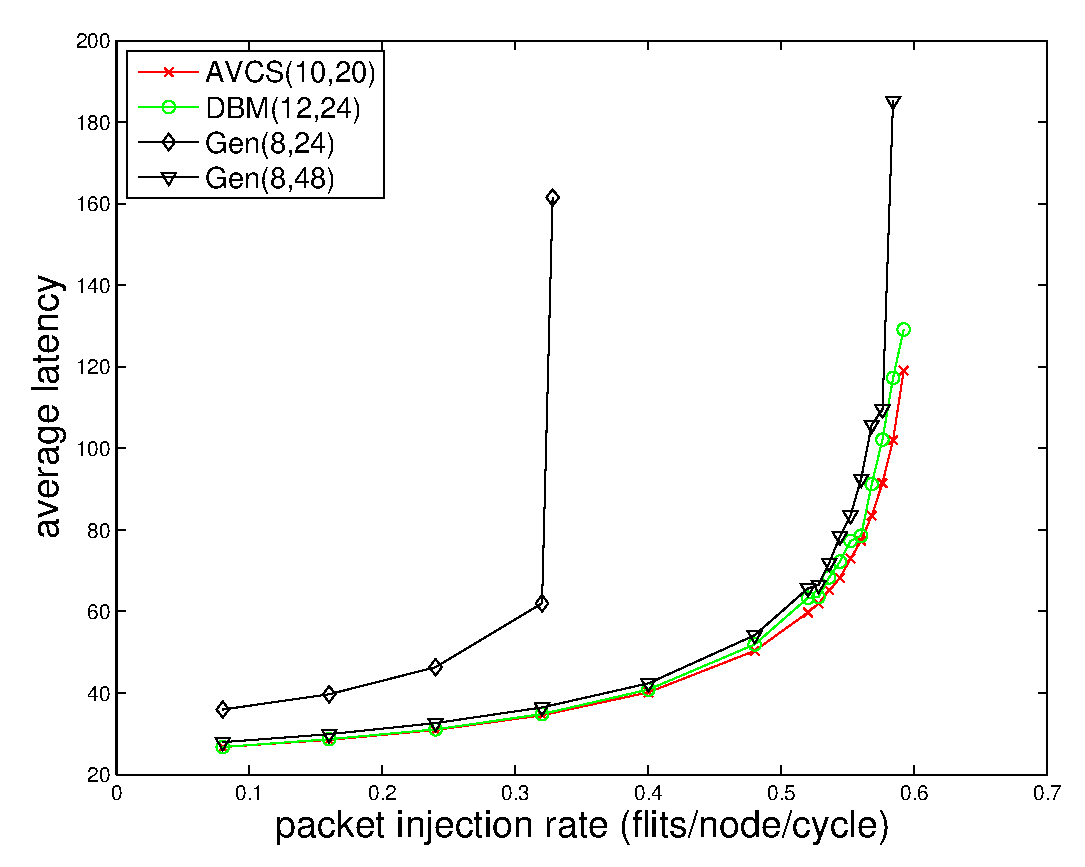
\includegraphics[scale=0.4]{figures/randomlat.eps}
  \caption{Latency comparison under random traffic pattern}\label{randomlat}
\end{figure}

\subsubsection{Realistic Traffic}
For the realistic applications, the workload of each router port is different and changes with time. Our proposal can adapt this dynamical change and allocate more buffer and VC resources to meet the resource requirement of input ports with higher traffic load. This property makes our approach more promising than the other two router architectures. We take two real-world applications, i.e. Video Object Plan Decoder (VOPD) \cite{6553191} and Multi-Window Display (MWD) \cite{1374853}, as examples to compare the performance of our proposal with Gen(8,24), Gen(8,48) and DBM(12,24). These two applications are mapped to $4\times 4$ and $4\times 3$ mesh NoC, as shown in Fig. \ref{vopd} and Fig. \ref{mwd}. The communication rate (flits/cycle) is labelled on the channel connecting two routers.
\begin{figure}[h]
  \centering
  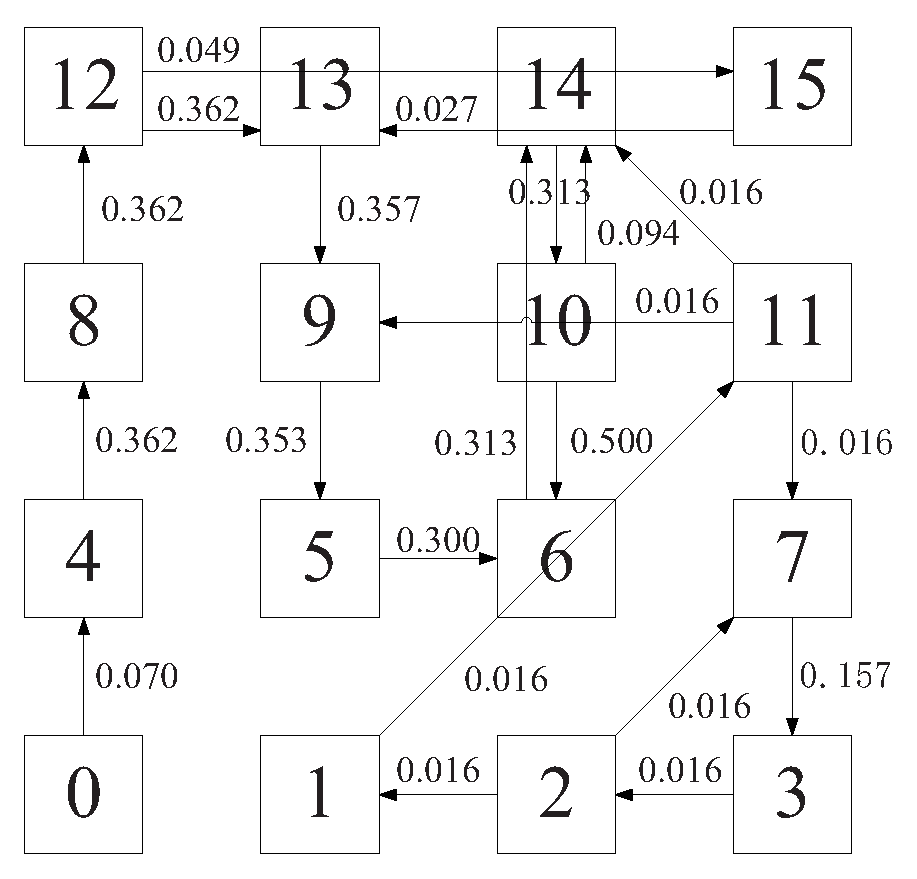
\includegraphics[scale=0.4]{figures/vopd.eps}
  \caption{Task mapping of VOPD application}\label{vopd}
\end{figure}
\begin{figure}[h]
  \centering
  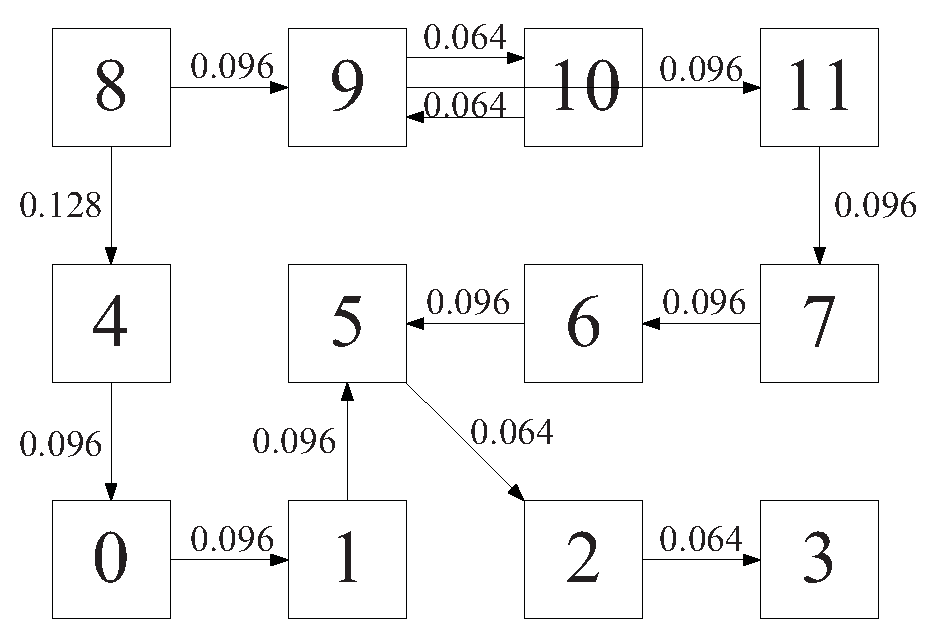
\includegraphics[scale=0.4]{figures/mwd.eps}
  \caption{Task mapping of MWD application}\label{mwd}
\end{figure}

For the given configuration listed in Table \ref{configure}, we run the simulation with the detailed RTL implementation of these three router architectures for all these applications. The experimental are presented in Table \ref{realisticapp}.
\begin{table}[h]
  \centering\caption{Simulation configuration}\label{configure}
  \begin{tabular}{|c|c||c|c|}
    \hline
    Topology & $4\times 4$ mesh  &   routing algorithm & DOR\\
    \hline
    Packet length & 10 flits & warmup period &   $1\times 10^4$ cycles\\
    \hline
    threshold & 1 cycle & sampling period &   $1\times 10^5$ cycles\\
    \hline
    \end{tabular}
\end{table}

The experimental results show that, AVCS achieves better performance than LLB(12,24), Gen(8,24) and Gen(8,48). This is because our structure improves the buffer utilization and reduces the blocking caused by VC insufficiency, which makes it possible to achieve better performance by utilizing fewer buffer space.
\begin{table}[h]
  \centering\caption{Average latency comparison (in cycles)}\label{realisticapp}
\begin{tabular}{|c|c|c|c|}
\hline
 & VOPD & MWD\\
 \hline
AVCS(10,20) & 29.3805 & 22.4489\\
\hline
Gen(8,24) & 606.31 ($\downarrow$ 95.2\%) & 30.0246 ($\downarrow$ 25.2\%)\\
\hline
Gen(8,48) & 29.9462 ($\downarrow$ 1.9\%) & 22.5405 ($\downarrow$ 0.4\%)\\
\hline
DBM(12,24) & 29.5593 ($\downarrow$ 0.6\%) & 22.4777 ($\downarrow$ 0.1\%)\\
\hline
\end{tabular}
\end{table}

\subsection{Power and Area Comparison}\label{area}
The detailed RTL implementation of AVCS and typical router are synthesized with Synopsys Design Compiler under FreePDK 45nm standard cell library \cite{nangate}. We configure medium effort optimization option for the synthesis tool and set the working voltage and frequency to 1.1V and 200MHz. For AVCS(10,20) router, the power consumption with assumed switching activity factor 10\% is 141.445 mW, chip area is 1002486.625 $\mu^2 m$. In contrast, Gen(8,48) consumes 208.224 mW power and occupies 1135084.5 $\mu^2 m$ chip area under the same conditions, which saves 11.7\% chip area and reduces 32.1\% power consumption. We compared the power and area overhead of AVCS(10,24) with Gen(8,48) since they achieves the similar performance under both synthesis and realistic traffic patterns.

Finally, we compared the chip area and power consumption of our revised VCA and SWA with that of used in typical router. Supposing each router has $P$ input ports and each port has $V$ VCs. Then, a $PV\times PV$ VCA and a $PV\times P$ SWA should be deployed in typical router, while our approach uses a $5/6PV\times 5/6PV$ VCA and a $5/6PV\times P$ SWA instead. We let $P=5$ and change V from 6 to 24 with step 6, the power and chip area of these two schemes are listed in Table \ref{alloccost1} and Table \ref{alloccost2}, respectively. As shown in Table \ref{alloccost1}, our approach saves more chip area than the typical allocator structure. In addition, our approach tends to save more power consumption than the baseline allocator structure when the more VCs are supported.
\begin{table}[h]
\centering\caption{Chip area comparison with baseline allocator}\label{alloccost1}
\begin{tabular}{|c|c|c|c|c|}
\hline
\multirow{2}{*}{$\#$VC} & \multicolumn{3}{|c|}{Area($\mu m^2$)}\\
\cline{2-4}
& Baseline & AVCS & AVCS vs. Baseline\\
\hline
6 & 62013.8828 & 58659.8906 & $\downarrow$ 5.4\%\\
\hline
12 & 221112.5312 & 206178.4062 & $\downarrow$ 6.8\%\\
\hline
18 & 492946.6562 & 426018.5625 & $\downarrow$ 13.6\%\\
\hline
24 & 882065.3750 & 822519.5000 & $\downarrow$ 6.8\%\\
\hline
\end{tabular}
\end{table}
\begin{table}[h]
\centering\caption{Power comparison with baseline allocator}\label{alloccost2}
\begin{tabular}{|c|c|c|c|c|}
\hline
\multirow{2}{*}{$\#$VC} & \multicolumn{3}{|c|}{Power(mW)}\\
\cline{2-4}
& Baseline & AVCS & AVCS vs. Baseline\\
\hline
6 & 5.846 & 6.292 & $\uparrow$ 7.6\%\\
\hline
12 & 14.916 & 15.276 & $\uparrow$ 2.4\%\\
\hline
18 & 26.962 & 24.870 & $\downarrow$ 7.8\%\\
\hline
24 & 38.999 & 38.732 & $\downarrow$ 0.7\%\\
\hline
\end{tabular}
\end{table}

\section{conclusion and future works}\label{conc}
The buffer organization and management scheme is a key factor which determines the performance of wormhole-switched NoC router. In this paper, we propose a runtime adaptive buffer and VC sharing approach, which dynamically allocates the shared buffer and VCs to the desired input ports to better adapt the traffic condition and improve the network performance. Comparing with existing UBS and LLS approaches, our method introduces the lest hardware overhead and further improve the network performance. Another contribution of this paper is that we proposed the idea of request port sharing, which uses a smaller VCA and SWA to perform the VC and switch allocation. By applying this sharing scheme, the chip area and power overhead of these two components are reduced significantly. The synthesis results show that our approach saves 32.1\% power and 11.7\% chip area while comparing with typical router of the similar performance. For the future work, we plan to realize the fault tolerant and QoS isolation in this architecture.

\section*{Acknowledgment}
The authors thank the reviewers for their suggestions and comments, and all the experiments are carried out at the Integrated Microsystem Lab (IML) of McGill University. This research is supported by High Technology Research and Development Program of China (Grant No. 2012AA012201, 2012AA011902).

\bibliographystyle{ieicetr}% bib style
\bibliography{Docear}% your bib database

%\begin{thebibliography}{99}% more than 9 --> 99 / less than 10 --> 9
%\bibitem{}
%\end{thebibliography}

\profile[figures/me.eps]{Baoliang Li}{ was born in 1987. He received the B.S. degree in Computer Science and Technology from Tsinghua University, P.R. China, in 2009. He is currently working towards the Ph.D. degree from College of Computer at National University of Defense Technology (NUDT), P.R. China. His research interests is performance analysis of computer networks and Networks-on-Chip, with a special interest on the analytical methods of network calculus.}
\profile[figures/fqy.eps]{Quanyou Feng}{was born in 1982. He received the B.S. degree from Tsinghua University (Beijing, 100084, P. R. China) in Sep. 2005 and the M.S. degree in computer science and technology from National University of Defense Technology (NUDT), China, in 2008. His research focuses on high-performance computing and interconnection networks.}
\profile[figures/dwh.eps]{Wenhua Dou}{ was born in 1946. He received the B.S. degree in computer science from Harbin Military Engineering College in 1970. He has been working at National University of Defense Technology (NUDT), P.R. China since 1970. He was vice dean of College of Computer, NUDT from 1999 to 2003. He is currently a professor of College of Computer, NUDT with research focusing on computer networks.}
%\profile*{}{}% without picture of author's face

\end{document}
